\section{Choice of drone}\label{s:vores_drone}
For the purpose of this project a multirotor drone will be chosen. Since the unavailability of the drones at the university, the group members get the opportunity to order the drone in collaboration with the supervisors and hobbyking.dk. A Quanum Outlaw 270 Racing Drone Frame Kit with 305 mm in diameter is chosen as the main body for the drone system as shown on figure \ref{fig:TheChosenOne}. The reason for choosing a larger drone body and the reason for more powerful motors will be used is because of the possibility of lifting a heavier payload, such as an Arduino and sensors. 

\begin{figure}[H]
    \centering
    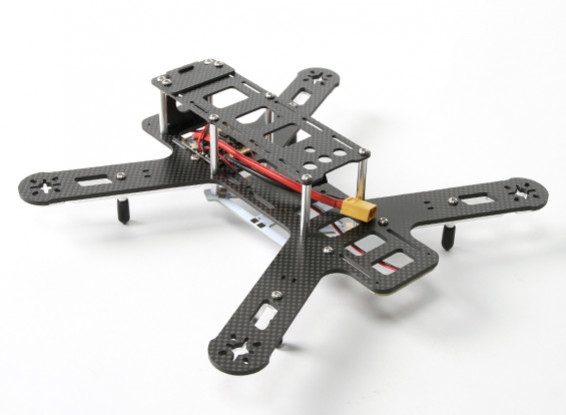
\includegraphics[width=0.5\textwidth]{figures/ch_intro/TheChosenOne.jpg}
    \caption{A picture of the chosen drone for this project}
    \label{fig:TheChosenOne}
\end{figure}

\subsection*{Composition of quadcopter parts}
The composition of the quadcopters different parts is illustrated in figure \ref{fig:blockdiagramDrone}, where the flight controller is connected to the radio receiver and getting user information for how the drone should move. The flight controller then sends a signal to the ESC’s (Electronic Speed Controller) of how fast the motors should rotate.

\begin{figure}[H]
    \centering
    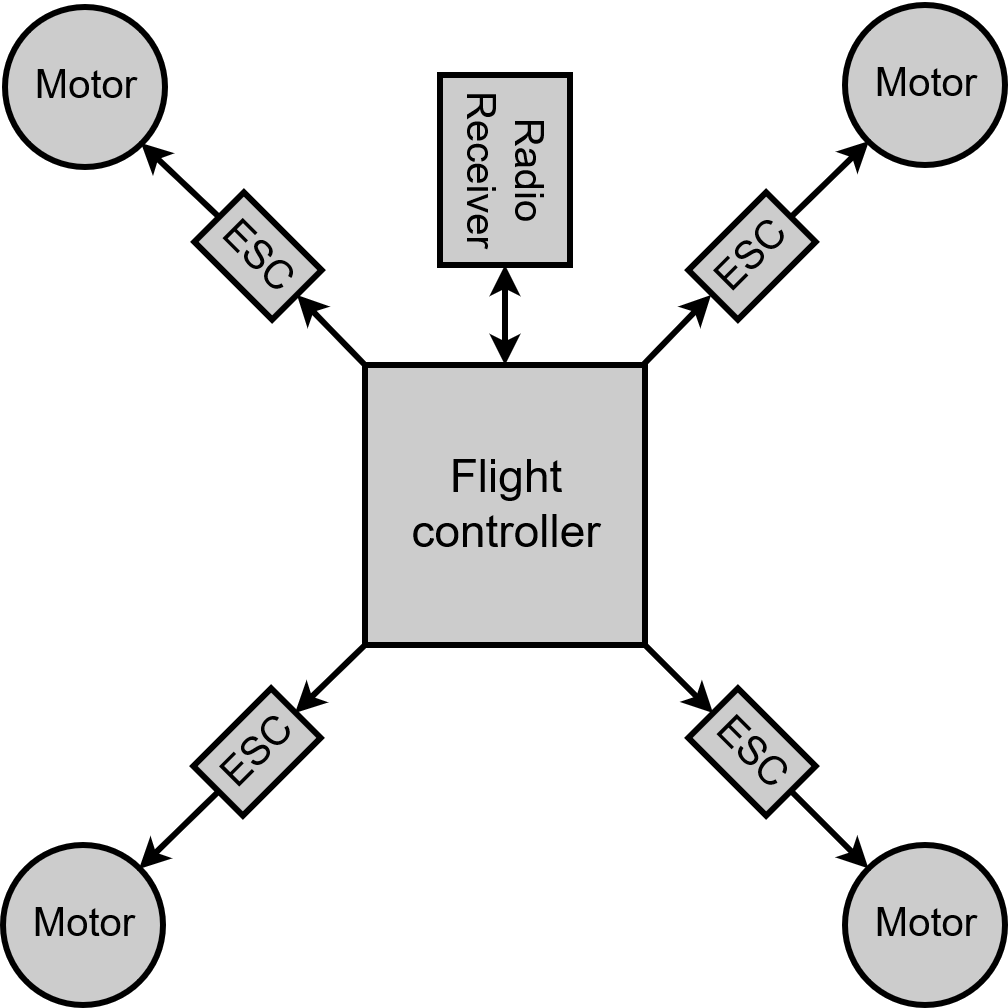
\includegraphics[width=0.5\textwidth]{figures/ch_intro/BlockdiagramOfTheDrone.png}
    \caption{Block diagram of the quadcopters individual parts connection}
    \label{fig:blockdiagramDrone}
\end{figure}

\begin{table}[H]
\begin{tabular}{|c|l|}
\hline
\textbf{Quantity} & \textbf{Item} \\ \hline
1 x  & \textbf{Frame kit:} Quanum Outlaw 270 Racing Drone Frame Kit \\ \hline
1 x & \textbf{Flight controller:} Skyline32 Acro Flight Controller w/Baseflight  Cleanflight \\ \hline
6 x & \textbf{Motor:} MultiStar Viking 2206-2600kv Brushless Outrunner Drone Racing Motor (CCW) \\ \hline
4 x & \textbf{Battery} Turnigy Heavy Duty 2200mAh 4S 60C Lipo Pack w/XT60U Connector \\ \hline
1 x & \textbf{Controller unit} Turnigy TGY-i6 AFHDS Transmitter and 6CH Receiver (Mode 2) \\ \hline
6 x & Turnigy MultiStar 32bit 30A Race Spec ESC 2~4S NAKED (OPTO) \\ \hline
20 x & \textbf{Propellers:} Diatone Bull Nose Plastic Propellers \\ \hline
\end{tabular}
\end{table}